\documentclass{article}
\usepackage[a4paper, top=3cm, bottom=2.5cm, left=2.5cm, right=2.5cm]{geometry}
\usepackage[spanish]{babel}
\usepackage[utf8]{inputenc}
\usepackage{tikz}
\usepackage{titling}
\usepackage{graphicx}
\usepackage{fancyhdr}
\usepackage{amsmath}
\usepackage{amssymb}
\usepackage{multicol}
\usepackage{cancel}
\usepackage{setspace}
\usepackage{pgfplots}
\usepackage{hyperref}
\usepackage{float}
\pgfplotsset{compat=1.18}
\setlength{\parskip}{1em}
\setlength{\parindent}{0pt}


\pagestyle{fancy}
\fancyhf{}
\fancyhead[L]{
\includegraphics[width=2cm]{assets/logo-utp.png}}
\fancyhead[R]{\textbf{Introducción a las TIC}}

\fancyfoot[R]{\thepage}

\setlength{\textheight}{23cm}

\setlength{\headheight}{17.26935pt}
\addtolength{\topmargin}{-5.26935pt}
\setlength{\textheight}{23cm}


\title{
  
\includegraphics[width=5cm]{./assets/logo-utp.png} \\
  \vspace{1cm}
  \textbf{Universidad Tecnológica del Perú} \\
  \vspace{2cm}
  \textbf{Implementación de Soluciones TIC para la Optimización Operativa en la Bodega Morocco} \\
  \vspace{1cm}
  \large \textbf{Para el curso de Introducción a las Tecnologías de la Información y Comunicación} \\
}
\author{
  \begin{tabular}{ll}
    \textbf{Luis Huatay Salcedo.} & \texttt{hsluis4326@gmail.com} \\
    \textbf{Carlos Huari.} & \texttt{carlosplop123@gmail.com} \\
    \textbf{Jhocelin Jimenez.} & \texttt{nicollj49@gmail.com} \\
    \textbf{Eva Larico.} & \texttt{evalarico073@gmail.com} \\
    \textbf{Kelvin Lázaro.} & \texttt{kelvinelb@gmail.com} \\
  \end{tabular} \\\\
  \texttt{Sección 24240}
}


% ENVIROMENTS

\begin{document}
\newgeometry{top=4cm}
\maketitle
\begin{center}
Docente Mg. Mattos Quevedo, Juan Manuel
\end{center}
\restoregeometry

\newpage 

\tableofcontents

\newpage

\section{Marco Teórico}

  \subsection{Definición de TIC}

    Las Tecnologías de la Información y Comunicación (TIC) son un conjunto de herramientas, recursos y sistemas que permiten la adquisición, almacenamiento, procesamiento, transmisión y presentación de información de manera digital. Estas tecnologías han revolucionado la forma en que las personas se comunican, acceden a la información y realizan sus actividades diarias, transformando la sociedad y la economía en un entorno cada vez más digitalizado.

    Según Huidobro J. (2007) Se entiende un termino dilatado empleado para designar lo relativo a la informática conectada a Internet, y especialmente el aspecto social de éstos. Ya que Las nuevas tecnologías de la información y comunicación designan a la vez un conjunto de innovaciones tecnológicas pero también las herramientas que permiten una redefinición radical del funcionamiento de la sociedad.

    \begin{flushright}
      \textit{Huidobro J. (2007). Tecnologías de la información y la comunicación.}
    \end{flushright}



  \subsection{Importancia de las TIC}

    Las Tecnologías de la Información y Comunicación (TIC) juegan un papel fundamental en la sociedad actual, ya que han transformado la forma en que las personas se comunican, trabajan, estudian, se divierten y realizan sus actividades diarias. Algunas de las razones por las que las TIC son importantes son las siguientes:

    \begin{itemize}
      \item \textbf{Facilitan la comunicación:} Las TIC permiten a las personas comunicarse de forma rápida, eficiente y económica a través de diversos medios, como el correo electrónico, las redes sociales, las llamadas telefónicas, los mensajes de texto, entre otros. Esto ha acortado las distancias y ha facilitado la interacción entre individuos, empresas, organizaciones y gobiernos en todo el mundo.

      \item \textbf{Mejoran el acceso a la información:} Las TIC han democratizado el acceso a la información al permitir a las personas buscar, compartir y acceder a una amplia variedad de contenidos en línea. Esto ha contribuido a la educación, la investigación, el entreten
      \item \textbf{Facilitan el trabajo colaborativo:} Las TIC permiten a las personas trabajar de forma colaborativa en tiempo real, independientemente de su ubicación geográfica. Herramientas como el correo electrónico, los sistemas de gestión de proyectos, las videoconferencias y las plataformas de colaboración en línea facilitan la comunicación y la coordinación entre equipos de trabajo.
      
      \item \textbf{Optimizan los procesos empresariales:} Las TIC han revolucionado la forma en que las empresas operan al permitir la automatización de procesos, la gestión eficiente de la información, la toma de decisiones basada en datos y la mejora de la productividad. Esto ha llevado a la creación de nuevos modelos de negocio, la optimización de tareas y la generación de nuevas oportunidades en el mercado.
      
      \item \textbf{Fomentan la innovación:} Las TIC son un motor de innovación en la sociedad al permitir el desarrollo de nuevas tecnologías, aplicaciones y servicios que mejoran la calidad de vida de las personas, impulsan el crecimiento económico y promueven el desarrollo sostenible. La tecnología ha transformado sectores como la salud, la educación, el transporte, la energía, la agricultura, entre otros, generando impactos positivos en la sociedad.
    \end{itemize}

\newpage 

\subsection{Antecedentes}

\textbf{\textit{Implementación del sistema de ventas e inventario en Comercial Juanita, Aguas Verdes - Tumbes; 2021}}

De acuerdo a Silva P. (2022). Comercial Juanita, es una empresa dedicada a la venta de productos agropecuarios, que se ha visto enfrentando a diversos desafíos al trabajar con un ineficiente sistema manual de ventas e inventario. El informe presente describirá todos los problemas encontrados en el negocio utilizando el sistema tradicional, tanto así, como las soluciones tecnológicas (TIC) que se implementaron para optimizar la eficiencia operativa. 

\begin{itemize}
  \item \textbf{Problemas identificados:} 
  \begin{enumerate}
    \item \textbf{Registro manual de ventas:} Comercial Juanita, manejaba las ventas y el inventario mediante registros en cuadernos. Este método manual presentaba un gran riesgo ya que toda la información era almacenada en una libreta de apuntes, ocasionando así, confusiones y disgustos al cliente. Además, el rápido deterioro de los cuadernos presentaba un gran riesgo por la pérdida de datos. 
    \item \textbf{Confusiones y Errores en el inventario del negocio:} El sistema manual generaba muchos errores ya que no contaba con un control estructurado de los productos en su inventario. Esta falta de control de su inventario generaba confusión entre los empleados y muchas demoras en el proceso de venta, afectando a la satisfacción del cliente.   
    \item \textbf{Falta de un sistema de control:} Al depender netamente de registros físicos, no contaba con un mecanismo seguro para controlar el sistema de inventario o al menos garantizar la exactitud de la información. Este problema limitaba el seguimiento de ventas y el inventario, haciendo más frecuente la aparición de errores que afectaran sus operaciones diarias o su relación con su clientela. 
  \end{enumerate}
  \item \textbf{Herrmientas TIC implementadas:}
  \begin{enumerate}
    \item \textbf{Automatización de los procesos de venta:} Al implementar las TIC permitió la automatización de los registros de ventas y mejorar la gestión del inventario, eliminando la necesidad de registros manuales. Con un nuevo sistema, los datos se almacenan de manera digital, mejorando asi la eficiencia y la consulta de información 
    \item \textbf{Mejora en la eficiencia y rapidez:} Al implementar las TIC, redujo significativamente el tiempo de atención al cliente, debido al rápido acceso a los datos del inventario y también a que los empleados puedan visualizar en tiempo real a la disponibilidad de los productos. 
    \item \textbf{Sistema Centralizado de Inventario Seguro:} El nuevo sistema cuenta con una base de datos que centraliza toda la información de ventas e inventario. Este cambio facilita el almacenamiento del historial de sus clientes y todas sus compras, tambien permite un control efectivo de los productos disponibles. La empresa ahora puede rastrear las transacciones de forma segura, minimizando los errores y reforzando la seguridad de su información.  
    \item \textbf{Metodología utilizada:} Comercial Juanita utilizo la metodología RUP (Rational Unifed Process) y UML (Lenguaje unificado de modelado). Estas metodologías estructuran y organizan todos los procesos del sistema, permitiendo un diseño adecuado de la base de datos y de interfaces de usuario. 
  \end{enumerate} 
\end{itemize}



\newpage

\section{Descripción de la Empresa}

  \begin{spacing}{1.5}
    \noindent
    \textbf{Nombre de la Empresa:} Bodega Morocco \\
    \textbf{Giro de la Empresa:} Venta de productos de primera necesidad \\
    \textbf{Correo Electrónico:} bodegaMorocco@gmail.com \\
    \textbf{Teléfono:} 987654321
  \end{spacing}

  La Bodega Morocco es un negocio familiar que ha servido a la comunidad de San Juan de Miraflores, específicamente en el sector 12 de noviembre de Pamplona Alta, por más de una década. A pesar de su tamaño modesto, la bodega ha logrado ganarse la confianza de los vecinos por su atención cercana y productos de calidad. El establecimiento ofrece una variedad de productos básicos que cubren las necesidades diarias de sus clientes, tales como arroz, azúcar, bebidas, enlatados y productos de limpieza. Estos productos son esenciales para los hogares de la zona, y la atención al cliente es únicamente presencial, lo que refuerza la relación directa con su clientela.

  Actualmente, la Bodega Morocco opera desde un único local. A pesar de las limitaciones en infraestructura, los dueños buscan constantemente mejorar sus servicios para agilizar los procesos de compra y brindar una mejor experiencia a sus clientes. La bodega ha experimentado un crecimiento constante en los últimos años, lo que ha llevado a los dueños a considerar la posibilidad de expandir su negocio. Sin embargo, antes de tomar esta decisión, desean optimizar sus operaciones actuales para garantizar que puedan manejar un mayor volumen de ventas sin comprometer la calidad de su servicio.

\section{Problemática}

  La Bodega Morocco enfrenta varios desafíos en su operación diaria que limitan su capacidad de crecimiento y la calidad de su servicio. A continuación, se escogió uno de los problemas más críticos que afectan a la bodega y que se busca resolver con la implementación de soluciones TIC.

  \subsection{Procesos Manuales de venta e inventario:}

  Actualmente, la Bodega Morocco enfrenta una serie de desafíos relacionados con la gestión manual de sus ventas y la falta de un control de inventario adecuado. Los propietarios llevan un registro manual de las transacciones diarias, lo que implica un proceso laborioso, propenso a errores y que consume un tiempo considerable. Esta metodología limita su capacidad para tomar decisiones rápidas y eficaces sobre las compras y la reposición de productos.

  La ausencia de un sistema automatizado de inventario complica aún más la identificación de los artículos que se están agotando o aquellos con alta demanda. Esto puede resultar en una pérdida de oportunidades de venta y en la insatisfacción de los clientes al no encontrar productos disponibles. Además, la falta de un sistema digital impide analizar patrones de consumo, lo que dificulta la planificación de compras futuras. Sin una visión clara de los productos con mayor o menor rotación, es más probable que se acumulen productos no vendidos o se agoten artículos esenciales, afectando tanto la calidad del servicio como la satisfacción del cliente.

\newpage

\section{Objetivo}

  \begin{spacing}{1.5}
    \noindent
    \textbf{Objetivo General:} 
    
    Automatizar el registro de ventas y la gestión de inventario de la Bodega Morocco. Con esta solución se busca reducir significativamente el tiempo empleado en los procesos manuales y minimizar los errores que suelen ocurrir al realizar estas tareas de forma no automatizada. Implementar un sistema digital permitirá a los dueños de la bodega llevar un control más preciso y eficiente de sus ventas diarias, así como obtener una visión clara del estado del inventario. Esto facilitará la toma de decisiones informadas en cuanto a la reposición de productos, evitando tanto la falta de stock como la acumulación innecesaria de mercancías.

    \textbf{Objetivos Específicos:}
    \begin{itemize}
      \item Implementar un sistema de bases de datos para almacenar información sobre los productos, las ventas y el inventario de la bodega.
      \item Desarrollar una interfaz de usuario intuitiva y fácil de usar para registrar las ventas y actualizar el inventario de forma automatizada.
      \item Generar reportes periódicos sobre las ventas, el inventario y los productos más vendidos para facilitar la toma de decisiones.
      \item Capacitar al personal de la bodega en el uso del nuevo sistema y brindar soporte técnico continuo para garantizar su correcto funcionamiento.
      \item Evaluar el impacto de la implementación de la solución TIC en la eficiencia operativa de la bodega y en la satisfacción del cliente.
    \end{itemize}
  \end{spacing}

\newpage

\section{Herramientas TIC a Emplear}

  Para la implementación de la solución propuesta, se utilizarán las siguientes herramientas TIC:

  \subsection{Sistema de Gestión de Bases de Datos (SGBD):}

    Un Sistema de Gestión de Bases de Datos (SGBD) es un software que permite almacenar, organizar, recuperar y gestionar datos de forma eficiente y segura. En el caso de la Bodega Morocco, se utilizará un SGBD para almacenar información sobre los productos, las ventas y el inventario de la bodega. Esto permitirá a los propietarios acceder a los datos de forma rápida y precisa, así como generar informes detallados sobre el desempeño del negocio.

  \subsection{Aplicación Web para Registro de Ventas:}

    Una Aplicación Web es un programa informático que se ejecuta en un navegador web y que permite a los usuarios interactuar con una base de datos a través de una interfaz gráfica. En este caso, se desarrollará una aplicación web para que los empleados de la bodega puedan registrar las ventas de forma automatizada. La aplicación permitirá ingresar los datos de los productos vendidos, calcular el monto total de la venta y actualizar el inventario de forma automática.

  \subsection{Sistema de Control de Inventario:}

    Un Sistema de Control de Inventario es una herramienta que permite llevar un registro detallado de los productos disponibles, las existencias actuales y las ventas realizadas. Este sistema se integrará con la aplicación web de registro de ventas para mantener actualizada la información del inventario en tiempo real. Los propietarios de la bodega podrán consultar el estado de los productos, identificar los artículos con mayor demanda y planificar las compras de reposición de forma más eficiente.

  \subsection{Generación de Reportes Automatizados:}

    La generación de reportes automatizados es una funcionalidad que permite extraer información relevante de la base de datos y presentarla de forma estructurada y visual. Se desarrollarán reportes periódicos sobre las ventas, el inventario y los productos más vendidos para facilitar la toma de decisiones de los propietarios de la bodega. Estos reportes proporcionarán una visión clara del desempeño del negocio y permitirán identificar oportunidades de mejora.

\newpage

\section{Prototipado de las soluciones}

A continuación se muestra un prototipo de login para el control del inventario de la Bodega Morocco. Esta aplicación web permitirá a los empleados de la bodega acceder al sistema de control de inventario y registrar las ventas de forma automatizada.

% imágenes:

\begin{figure}[H]
  \centering
  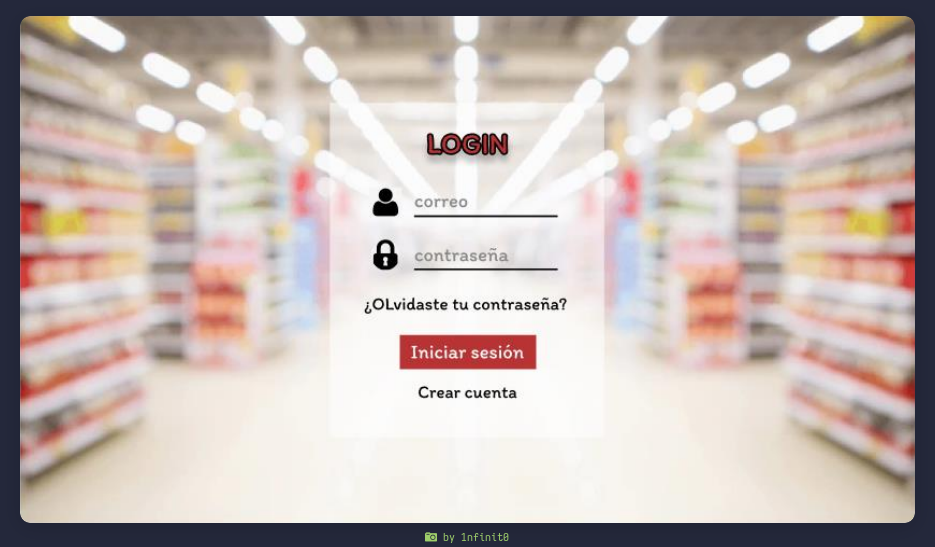
\includegraphics[width=0.8\textwidth]{./assets/login.png}
  \caption{Prototipo de Login}
\end{figure}

\begin{figure}[H]
  \centering
  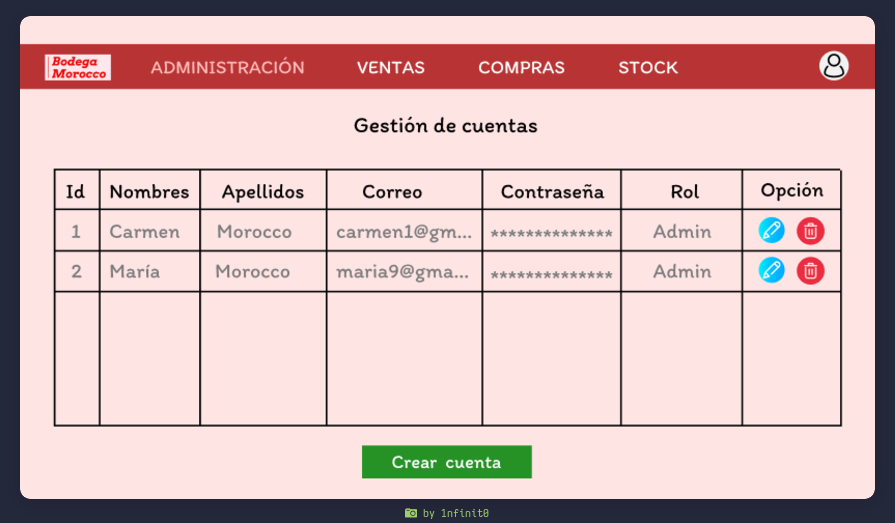
\includegraphics[width=0.8\textwidth]{./assets/bd.png}
  \caption{Vista de la Base de Datos}
\end{figure}

\newpage

\begin{thebibliography}{9}
  \addcontentsline{toc}{section}{Referencias}

  \bibitem{Huidobro}
  Huidobro J. (2007). Tecnologías de la información y la comunicación. Universidad Politénica de Madrid.

  \bibitem{Silva}
  Silva P. (2022). Implementación del sistema de ventas e inventario en Comercial Juanita, Aguas Verdes - Tumbes. Universidad Nacional de Tumbes.

\end{thebibliography}
\end{document}